\section{Resultater og analyser}
\label{sec:resultater}

\subsection{Utsnurring av svinghjulet}
\label{sec:res-utsnurring}
Utsnurringen er målt med ML-2 og behandlet som beskrevet i seksjon~\ref{sec:utsnurring-behandling}. Begge seriene er tatt 6.~november 2026, med fett i lagrene og trommel TR-1. Rådata ligger i mappen
\nolinkurl{Code/utsnurring_diagnose/data/}, og tabellene og figurene lages med \nolinkurl{Code/rapportfigurer.py}.

\subsubsection{Referanseserie med tannhjulet koblet}
I referanseserien griper pinjongen i tannhjulet, så drivakselen med de to drivhjulene snurrer med. Bilen er løftet, så hjulene går fritt. Serien har åtte opptrekk. Opptrekk 1 hadde omtrent \SI{1,8}{mN.m} tapsmoment, en tredjedel lavere enn de andre, uten at det er funnet noen forklaring. Det kan skyldes at noe satte seg etter at trommelen ble strammet. I opptrekk 5 hang løkka seg opp, og svinghjulet stoppet fra \SI{1080}{o/min} på under ett sekund. Begge er utelatt. De seks andre er vist i tabell~\ref{tab:utsnurring-koblet} og figur~\ref{fig:utsnurring-referanse}.

\begin{table}[H]
    \centering
    \caption{Utsnurring med tannhjulet koblet. Toppturtallet er rett etter at løkka slipper.}
    \label{tab:utsnurring-koblet}
    \small
    \renewcommand{\arraystretch}{1.3}
    \begin{tabular}{|c|c|c|c|c|}
        \hline
        \textbf{Opptrekk} & \textbf{Topp [o/min]} & \textbf{Til stopp [s]} & \textbf{1000 til 300 o/min [s]} & \textbf{Snittmoment [mN\,m]} \\
        \hline
        2 & 2166 & 3,88 & 1,66 & 2,66 \\
        3 & 2830 & 4,96 & 1,66 & 2,65 \\
        4 & 2281 & 4,20 & 1,61 & 2,74 \\
        6 & 3030 & 5,16 & 1,66 & 2,66 \\
        7 & 3125 & 4,76 & 1,56 & 2,83 \\
        8 & 2791 & 5,14 & 1,74 & 2,54 \\
        \hline
        \textbf{Snitt} & \textbf{2704 ± 394} & & \textbf{1,65 ± 0,06} & \textbf{2,68} \\
        \hline
    \end{tabular}
\end{table}

\begin{figure}[H]
    \centering
    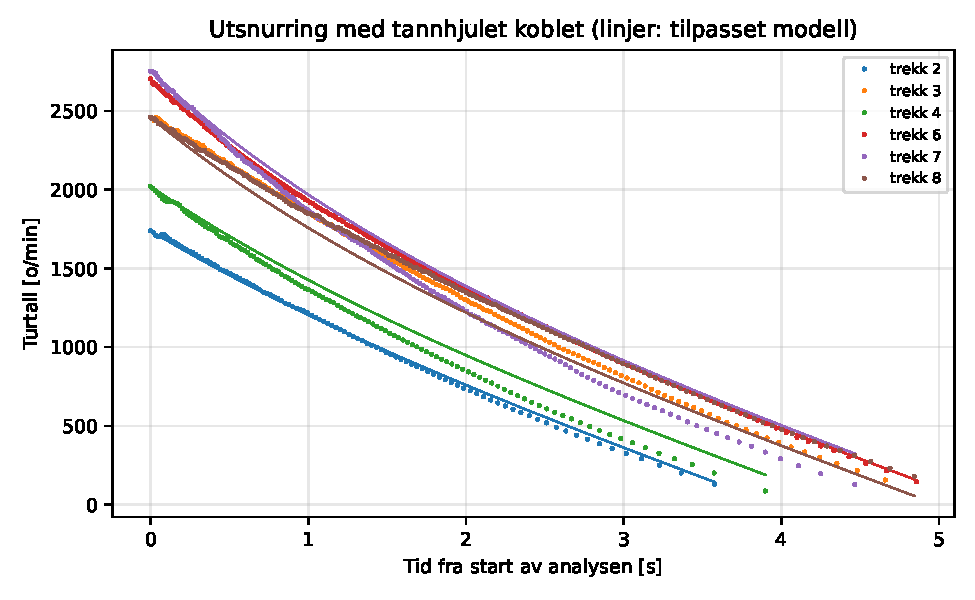
\includegraphics[width=0.7\textwidth]{Images/Maling/utsnurring_referanse.pdf}
    \caption{Utsnurring med tannhjulet koblet. Punktene er målt, og linjene er tapsmodellen tilpasset alle seks opptrekkene samtidig.}
    \label{fig:utsnurring-referanse}
\end{figure}

Tiden fra 1000 til \SI{300}{o/min} har et standardavvik på \SI{3,6}{\percent}, så målingen er godt repeterbar. Tapsmodellen tilpasset alle seks opptrekkene samtidig gir
\begin{equation}
    c_0 = \SI{2,35}{mN.m}, \qquad c_1 \approx 0, \qquad c_2 = \SI{4,3e-8}{N.m.s^2}.
    \label{eq:tapsmodell-maalt}
\end{equation}
Ved \SI{2700}{o/min} er de to leddene omtrent like store, \SI{2,35}{mN.m} og \SI{3,4}{mN.m}. Det konstante leddet er omtrent ti ganger det simuleringen antok fra før, $c_0 = \SI{0,2}{mN.m}$.

\subsubsection{Tannhjulet frakoblet}
For å skille tapet i svinghjullagrene fra tapet i tannhjulene og drivakselen ble tannhjulet koblet fra pinjongen. Serien har seks opptrekk. Opptrekk 1 er utelatt, fordi turtallet falt fra 2055 til \SI{1285}{o/min} på \SI{0,3}{s}, som tyder på at løkka hang seg opp. Resultatene er vist i tabell~\ref{tab:utsnurring-frakoblet}.

\begin{table}[H]
    \centering
    \caption{Utsnurring med tannhjulet frakoblet.}
    \label{tab:utsnurring-frakoblet}
    \small
    \renewcommand{\arraystretch}{1.3}
    \begin{tabular}{|c|c|c|c|c|}
        \hline
        \textbf{Opptrekk} & \textbf{Topp [o/min]} & \textbf{Til stopp [s]} & \textbf{1000 til 300 o/min [s]} & \textbf{Snittmoment [mN\,m]} \\
        \hline
        2 & 1709 & 6,97 & 3,27 & 1,35 \\
        3 & 1987 & 6,85 & 2,83 & 1,56 \\
        4 & 2362 & 5,56 & 2,40 & 1,83 \\
        5 & 2007 & 9,44 & 3,99 & 1,10 \\
        6 & 2335 & 5,65 & 2,17 & 2,03 \\
        \hline
        \textbf{Snitt} & \textbf{2080 ± 272} & & \textbf{2,93 ± 0,73} & \textbf{1,50} \\
        \hline
    \end{tabular}
\end{table}

Uten tannhjulet går svinghjulet lenger, men spredningen er \SI{25}{\percent} mot \SI{3,6}{\percent} i referanseserien. Figur~\ref{fig:tapsmoment} viser at hvert opptrekk holder et jevnt nivå hele veien ned, mens nivået varierer fra 1,1 til \SI{2,0}{mN.m} mellom opptrekkene. Spredningen er derfor ikke målestøy, men et tap som endrer seg fra gang til gang. Den sannsynlige årsaken er at svinghjulsakselen glir sideveis (seksjon~\ref{sec:problemlosning}). Ekstra gnissing kan bare øke tapet, så det laveste opptrekket, \SI{1,1}{mN.m}, er det beste anslaget for svinghjullagrene alene. Tannhjulene og drivakselen står da for omtrent $2{,}68 - 1{,}10 \approx \SI{1,6}{mN.m}$ av snittmomentet i referanseserien. Anslaget er usikkert til serien er gjentatt med avstandshylsene på plass.

\begin{figure}[H]
    \centering
    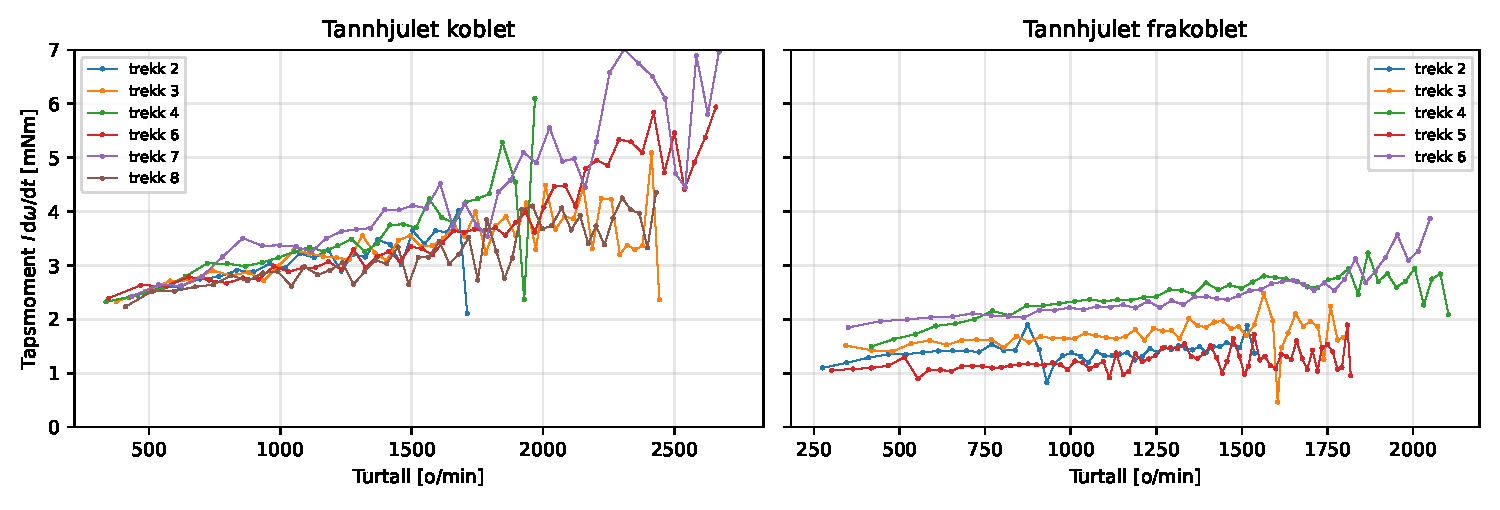
\includegraphics[width=\textwidth]{Images/Maling/tapsmoment.pdf}
    \caption{Tapsmoment mot turtall for hvert opptrekk, regnet fra stigningstallet til turtallskurven over åtte flanker.}
    \label{fig:tapsmoment}
\end{figure}

\subsubsection{Simulering med målte tap}
Figur~\ref{fig:sim-maalte-tap} viser simulert kjøredistanse med de antatte tapene og med tapsmodellen fra likning~\eqref{eq:tapsmodell-maalt}, både fra \SI{4000}{o/min} og fra \SI{2700}{o/min}, som er snittet for opptrekk med snor. Begge regner med Ø68-hjul og treghetsmomentet til fire hjul fra DH-2. Med antatte tap og \SI{4000}{o/min} kjører bilen \SI{35,4}{m} med $i = 4{,}29$. Med målte tap og \SI{2700}{o/min} kjører den \SI{3,1}{m} med samme utveksling, og beste utveksling flytter seg til $i \approx 3$ med \SI{3,3}{m}. Simuleringen fra \SI{4000}{o/min} med målte tap, \SI{5,1}{m}, bygger på et $c_2$-ledd som er ekstrapolert utenfor måleområdet.

\begin{figure}[H]
    \centering
    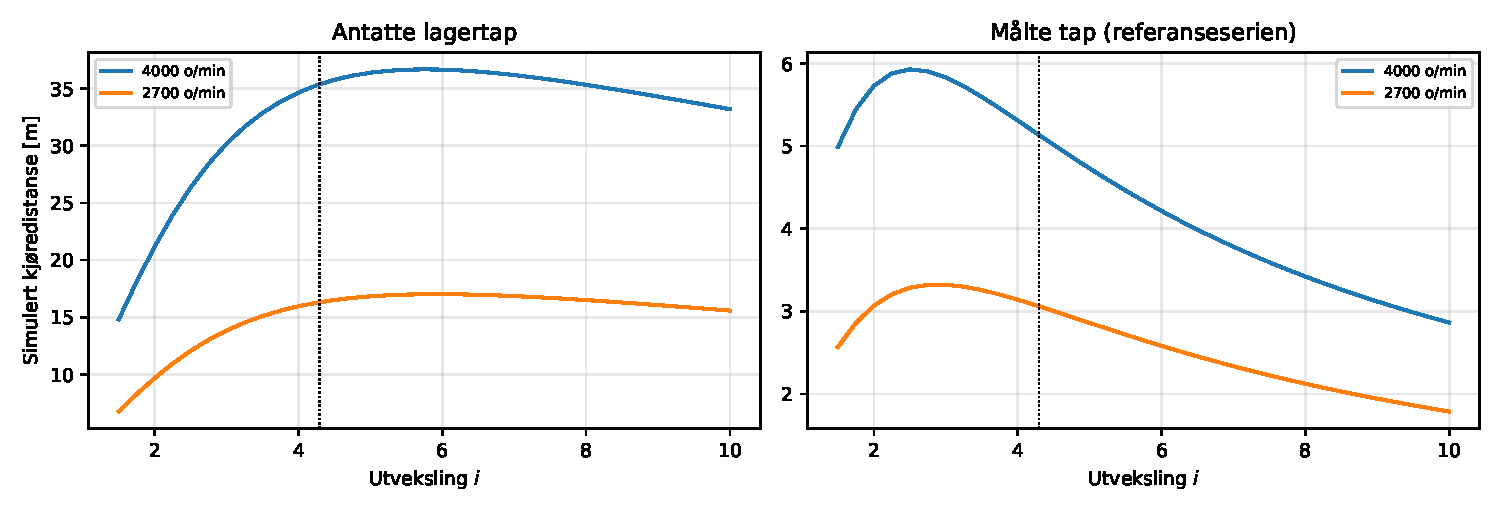
\includegraphics[width=\textwidth]{Images/Maling/sim_maalte_tap.pdf}
    \caption{Simulert kjøredistanse mot utveksling med antatte og målte tap. Den stiplede linjen er $i = 73/17 = 4{,}29$ fra DV-3.}
    \label{fig:sim-maalte-tap}
\end{figure}

\begin{comment}
% Testresultatene presenteres her. Tolkninger hører hjemme i diskusjonen.
\subsection{Funksjon og pålitelighet}
\subsection{Kjøredistanse og repeterbarhet}
\subsection{Retningsstabilitet og sammenligning av konfigurasjoner}
\subsection{Oppsummering av kravoppfyllelse}
% Fyll inn faktiske målinger, tabeller og figurer etter testing.
\end{comment}
